\chapter{Graph-Conditioned Diffusion Generator}
\label{ch:generator}

\section{Chapter Introduction and Design Rationale}
\label{sec:generator:introduction}

Chapter~\ref{ch:theory} identified a central difficulty in graph generation:
diffusion and score-based generative models provide stable denoising objectives
\citep{ho2020ddpm,song2020score}, but graphs are discrete, sparse,
permutation-sensitive, and subject to structural constraints
\citep{you2018graphrnn,niu2020permutation,vignac2022digress}. This chapter
addresses that difficulty by introducing the
\emph{Graph-Conditioned Diffusion Generator} (GCDG), the generator used in this
thesis.

GCDG separates continuous diffusion from discrete graph construction. A
conditional diffusion process is applied to padded node-level feature matrices,
while node existence, labels, degrees, pairwise edges, and edge labels are
predicted by dedicated modules before a constraint-aware decoder selects the
final graph. Throughout this chapter,
\emph{diffusion} refers to the forward corruption and reverse noise-removal
process over node-level features, while \emph{denoising} refers to the learned
prediction task performed inside that process.

The conditioning signal is a fixed graph-level vector \(C\). In this thesis,
\(C\) is instantiated using the \gls{nsppk} feature map introduced in
Chapter~\ref{ch:nsppk}, so neighbourhood, shortest-path, connector, and
attribute information can guide generation. The architecture itself only
requires a fixed-dimensional graph descriptor; other explicit graph descriptors,
graph kernels, or learned graph-level embeddings could therefore be substituted
\citep{costa2010fast,neumann2016propagation,borgwardt2020graphkernels,
hamilton2017graphsage,zhang2018endtoend,dwivedi2021graph}.

The setting considered here is graph-level-descriptor-to-graph generation. This
differs from unconditional generation, class-conditional generation, and
property-conditional generation, where the condition is often a class label or a
small set of scalar targets. It also differs from graph autoencoders and
variational graph autoencoders, which encode a specific input graph into a
sample-specific latent code before decoding it
\citep{kipf2016vgae,simonovsky2018graphvae}. GCDG receives only \(C\): when the
condition is computed from a reference graph, the target is not to reconstruct
that graph exactly, but to generate a graph that preserves information encoded
by the condition.
\begin{figure}[H]
    \centering
    \makebox[\textwidth][c]{%
    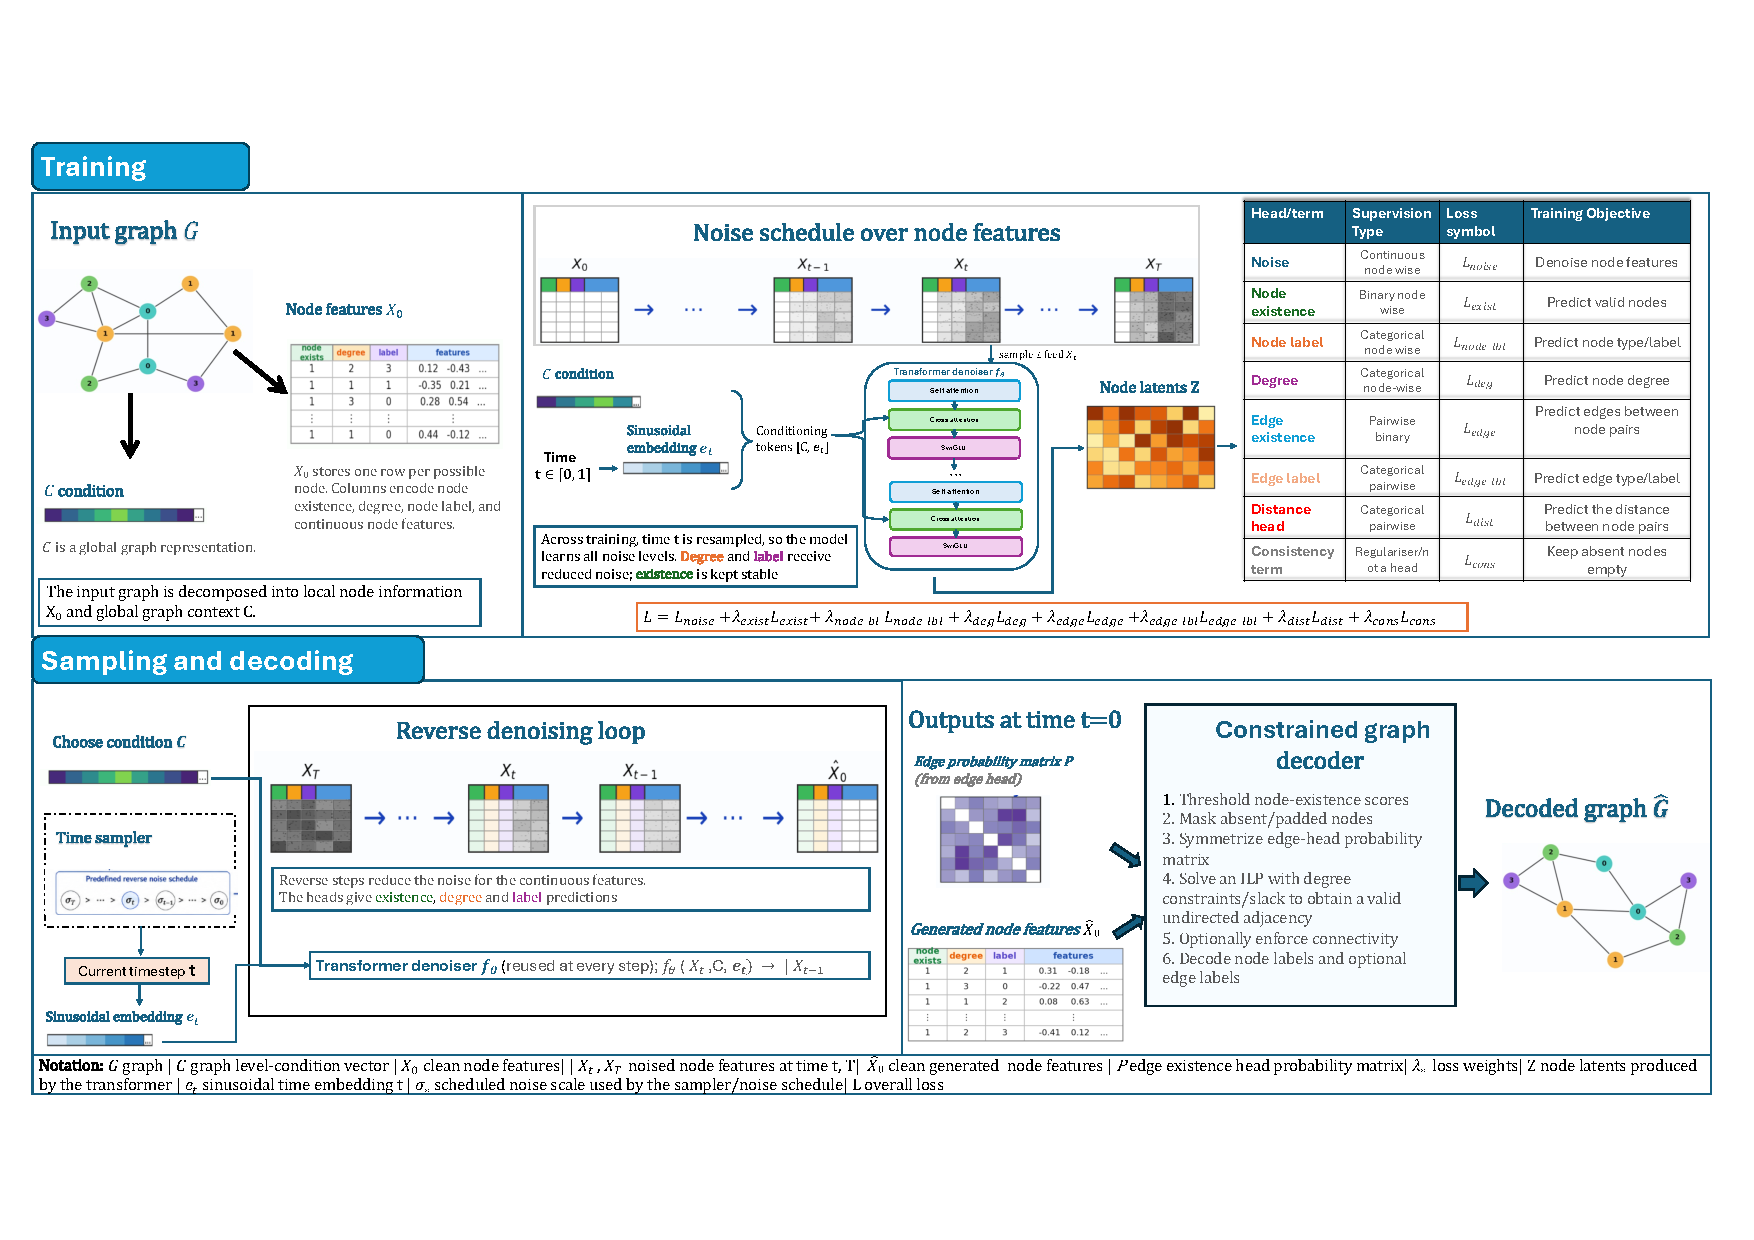
\includegraphics[
        width=1.25\textwidth,
        height=0.60\textheight,
        keepaspectratio,
        trim=0cm 2cm 0cm 2cm,
        clip
    ]{images/diffusion/pipeine_generator.pdf}
    }
    \caption{
    Overview of GCDG. The input graph is encoded into a padded node-level
    representation \(X_0\) and a graph-level condition vector \(C\). During
    training, a time \(t\) is sampled and noise is added to \(X_0\) according to
    a feature-wise schedule, producing \(X_t\). The conditional transformer
    receives \(X_t\), \(C\), and the time embedding \(e_t\), and produces
    node-level latents used by node-wise and pairwise prediction modules. At
    sampling time, a reverse noise schedule is followed from \(X_T\) to
    \(\hat X_0\), reusing the same denoising model at each step. The generated
    node representation and edge probability matrix are decoded into a graph by
    the constrained decoder.
    }
    \label{fig:generator:overview}
\end{figure}

The central contribution of this chapter is therefore the
graph-level-to-node-and-edge-level formulation. The model must translate a global structural
descriptor into the quantities needed to build a discrete graph: which nodes
exist, which labels and degrees they have, and which pairwise edges should be
selected. This is also distinct from direct graph diffusion models such as
DiGress, where the reverse process operates on categorical node and edge states
\citep{vignac2022digress}. In GCDG, the diffusion process acts on node-level
features, and graph topology is constructed through pairwise prediction and
constraint-aware decoding.

The rest of this chapter develops this staged generator in detail. It defines
the node-level representation, graph-level condition, diffusion architecture,
training objective, sampling procedure, and constraint-aware graph decoder.


\section{Method Overview and Representations}
\label{sec:generator:method-overview}


\subsection{Node-Level Feature Representation and Graph-Level Conditions}
\label{sec:generator:representation}

Let
\[
    G=(V,E,\tau_V,\tau_E)
\]
denote a finite, simple, undirected, discretely labelled graph, where
\[
    V=\{v_1,\ldots,v_n\},
    \qquad
    n=|V|,
\]
is the set of nodes and \(E\) is the set of edges. The functions
\[
    \tau_V:V\to\mathcal{T}_V
    \qquad\text{and}\qquad
    \tau_E:E\to\mathcal{T}_E
\]
assign discrete labels to nodes and edges, respectively. Let
\[
    K_V = |\mathcal{T}_V|
\]
denote the number of node-label classes.
In the terminology of Chapter~\ref{ch:theory}, these labels are categorical
node and edge attributes. The notation \(\tau_V,\tau_E\) is used deliberately
to avoid overloading the supervised-learning label space \(\mathcal{Y}\) or
the layer index \(\ell\) from the notation list.

The generator represents each graph at two complementary levels. At the graph
level, the default conditioning representation is obtained using the
\gls{nsppk} feature map introduced in Chapter~\ref{ch:nsppk}:

\[
    C
    =
    \phi_{\mathrm{NSPPK}}^{\mathrm{graph}}(G)
    \in
    \mathbb{R}^{d_C},
\]

where \(d_C\) is the dimension of the graph-condition vector. The vector \(C\)
summarises labelled neighbourhood patterns and broader structural relations in
\(G\), and is used as the graph-level description that conditions the denoising
process. This follows the graph-kernel view in which a graph is represented by
an explicit feature map \(\phi(G)\)
\citep{costa2010fast,borgwardt2005shortest,neumann2016propagation}. When the
resulting feature vector is high-dimensional, it may be compressed using a
dimensionality-reduction transformation, such as truncated \gls{svd}, fitted on
the training graphs. Once fitted, this transformation is held fixed: the same
projection is applied unchanged to training graphs, held-out condition graphs,
and generated graphs that are re-encoded for analysis.
The resulting graph-level condition vectors are also scaled using training-set
statistics. This scaling is fitted only on the training conditions and then
kept fixed, so held-out conditions and generated graphs are represented in the
same coordinate system.

Although \gls{nsppk} is the default condition encoder used in this thesis, the
generator architecture is not restricted to this particular feature map. More
generally, it requires a real-valued graph-level condition
\[
    \phi:\mathcal{G}\to\mathbb{R}^{d_C},
\]
where \(\mathcal{G}\) denotes the set of graphs considered in the task. Thus,
alternative explicit graph descriptors or learned graph-level embeddings can
replace \(\phi_{\mathrm{NSPPK}}^{\mathrm{graph}}\), provided that they produce a
compatible conditioning vector \(C\). Examples include learned graph
representations from graph neural networks or graph Transformers
\citep{hamilton2017graphsage,zhang2018endtoend,dwivedi2021graph}.

At the node level, the \gls{nsppk} node encoder produces a structural feature
vector for each node \(v_i\in V\):

\[
    r_i
    =
    \phi_{\mathrm{NSPPK}}^{\mathrm{node}}(v_i;G)
    \in
    \mathbb{R}^{d_r},
\]
Let $\mathcal{F}_i(G)$ denote the set of NSPPK feature occurrences assigned to
node $v_i$. The node-level structural representation is defined as
\[
r_i
=
\sum_{\xi\in\mathcal{F}_i(G)}
e_{h(\xi)}.
\]
where $h(\xi)$ is the hash bucket assigned to feature occurrence $\xi$ and
$e_{h(\xi)}$ is the corresponding standard basis vector.  At
a high level, \(r_i\) describes the labelled local structural context of node
\(v_i\), including the root-node label, labels of neighbouring nodes and
incident edges, rooted neighbourhood patterns over selected radii, and
relations between nearby neighbourhoods connected through short graph paths.
The representation is sparse and hash-based, so nodes with similar labelled
local structure activate similar feature dimensions.

The generator represents graphs with at most \(N_{\max}\) nodes, where
\(N_{\max}\) is fixed for a dataset or experimental setting. For each possible
node row \(i\in\{1,\ldots,N_{\max}\}\), the row of the node feature matrix is

\[
x_i
=
\left[
m_i;\,
g_i;\,
q_i;\,
r_i
\right]
\in\mathbb{R}^{d_{\mathrm{feat}}},
\]

Here $m_i\in\{0,1\}$ is the node-existence indicator and
\[
g_i=\deg(v_i)
\]
is the degree of node $v_i$ when row $i$ represents a real node. Before being
supplied to the denoising network, the degree coordinate is transformed using
the fitted node-feature scaler. For the auxiliary degree-prediction task, the
unscaled integer degree is treated as a categorical target in
\[
\{0,\ldots,D_{\max}\},
\]
where $D_{\max}$ is the maximum degree supported by the fitted model. The
degree-prediction head therefore has $D_{\max}+1$ output classes.

If degrees are clipped or grouped, the corresponding mapping is
defined by the experimental configuration.

\[
    q_i
    =
    \left[
        q_i^{(1)},\ldots,q_i^{(K_V)}
    \right]
    \in
    \{0,1\}^{K_V}
\]
is the one-hot encoding of the node label \(\tau_V(v_i)\). The final component
\(r_i\) contains the node-level \gls{nsppk} structural features. The
node-feature dimension is therefore
\[
    d_{\mathrm{feat}} = 2 + K_V + d_r.
\]
In the rest of this chapter, a \emph{feature component} refers to one scalar
entry or one contiguous block in this row vector: the existence component
\(m_i\), the degree component \(g_i\), the node-label one-hot block \(q_i\), or
the continuous structural representation \(r_i\).

The label vocabulary is learned from the training dataset and stored by the
encoder. Numeric labels, symbolic role labels, and molecular atom symbols are
all treated as unordered categorical classes. The decoder uses the stored
mapping to convert generated class indices back to the original node labels.
Since labels are discrete, the model predicts node-label logits and trains them
with cross-entropy over existing nodes; they are not reconstructed by scalar
regression.

Let \(N_{\max}\) denote the fixed row budget used for padding, chosen to cover
the largest graphs considered in a given experiment. The feature vectors are
stacked and padded to form the clean node feature matrix
\[
X_0
=
\begin{bmatrix}
x_1^\top\\
\vdots\\
x_n^\top\\
x_{n+1}^\top\\
\vdots\\
x_{N_{\max}}^\top
\end{bmatrix}
\in
\mathbb{R}^{N_{\max}\times d_{\mathrm{feat}}}.
\]


For a graph containing $n<N_{\max}$ nodes, rows $i>n$ represent padding rather
than real graph nodes. In these rows, $m_i=0$, while the remaining feature
components are assigned fixed padding values. Loss terms for degree, node
label, continuous reconstruction, and supervised node pairs use the existence
mask to exclude non-existent rows.

In the current implementation, padded rows remain present as transformer
tokens and are not removed by an attention padding mask. They may therefore
participate in intermediate self-attention computations, although they are
excluded from the masked training targets and from final graph decoding. This
fixed-row representation is retained consistently during training and
sampling.


Before the denoising model is trained, the continuous coordinates of the node
feature matrix are placed on a common numerical scale. The scaler is fitted on
real node rows from the training graphs, after any optional dimensionality
reduction of the structural feature block, and is then reused for validation
graphs, held-out reference graphs, and generated samples. Padding rows are not
used to fit this scaler. The node-existence component is kept as a binary indicator, rather
than being rescaled, because it is the mask that distinguishes real node rows
from padding rows. For notational simplicity, the equations below use \(X_0\)
for this internally scaled clean node feature matrix.

Because graph nodes do not have a canonical order, the row order in \(X_0\) is
an implementation choice rather than an intrinsic graph property. Two node
feature matrices that differ only by a simultaneous permutation of their rows
can represent the same labelled graph. The generator therefore uses two
training-time devices to reduce sensitivity to arbitrary row order. First, node
rows can be randomly permuted during training. Second, the clean-\(X_0\)
reconstruction loss can be evaluated after matching predicted rows to target
rows.

The matching step is a linear assignment problem. Given a predicted clean node
feature matrix \(\hat X_0\) and a target matrix \(X_0\), define a pairwise cost
between predicted row \(i\) and target row \(j\),
\[
c_{ij}
=
\left\|
B_{\mathrm{match}}
\odot
(\hat{x}_{0,i}-x_{0,j})
\right\|_2^2.
\]
where \(B_{\mathrm{match}}\) selects the continuous structural coordinates used
for matching. The matched target order is obtained by finding the permutation
\[
    \pi^\star
    =
    \arg\min_{\pi\in S_{N_{\max}}}
    \sum_{i=1}^{N_{\max}} c_{i,\pi(i)} .
\]
This is the classical assignment problem, solved in the implementation using
the Hungarian algorithm \citep{kuhn1955hungarian,munkres1957algorithms}. The
algorithm can be understood as finding the minimum-cost one-to-one pairing
between the predicted rows and the target rows. In this generator, the matching
cost deliberately excludes the existence, degree, and node-label components, so
the categorical prediction losses cannot choose an artificially favourable
alignment. The assignment itself is not a learned neural module and is not part
of sampling. It is a training alignment step: after \(\pi^\star\) is selected,
the usual losses compare the prediction with the permuted target rows.
The assignment is performed over the complete padded row set. Because the
existence component is excluded from the matching cost, the assignment does
not explicitly prevent a predicted real-node row from being matched to a
padded target row. The separate existence and categorical losses provide the
corresponding supervision.
The node feature matrix captures node existence, degree, node labels, and
node-level structural context. It does not directly specify the final adjacency
matrix.
Instead, edge existence and, when applicable, the discrete edge label
\[
    \tau_E(\{v_i,v_j\})
\]
are estimated separately for candidate node pairs by the pairwise prediction
module. The graph decoder then combines the generated node features and
pairwise edge predictions to construct the final discrete graph.

\section{Forward Diffusion and Corruption Process}
\label{sec:generator:forward}

During training, the clean node feature matrix \(X_0\) is corrupted at a
randomly sampled noise level. A time value

\[
    t \sim \mathcal{U}(0,1)
\]
is mapped to a noise scale

\[
    \sigma(t) = \sigma_{\min}
    + t(\sigma_{\max}-\sigma_{\min}).
\]
Gaussian noise is then added feature-wise:

\[
    X_t = X_0 + \Gamma(t) \odot \varepsilon,
    \qquad
    \varepsilon \sim \mathcal{N}(0,I),
\]
where \(\Gamma(t)\) contains the per-feature noise scales and \(\odot\) denotes
element-wise multiplication. This corruption process is not used in the same
way for every feature component. Continuous structural features are learned through a
denoising task, whereas node existence, degree class, and node-label attributes
are treated as supervised classification tasks. The model therefore does not ask
a single continuous reconstruction objective to recover all discrete quantities.
Instead, the training objective combines a continuous denoising loss for
real-valued feature dimensions with separate binary or categorical losses for the
discrete node attributes. The architectural modules that implement these
supervised losses are introduced in the next section.

For the categorical feature blocks, Gaussian perturbation is not the only
meaningful way to define a noisy input. A node label, for example, is not a
number whose value should be slightly increased or decreased; it is a class
membership. For this reason, the categorical part of the forward process can
also be defined as a discrete corruption task. The model is shown a corrupted
degree or node-label class at noise level \(t\), and the supervised target is
the original clean class from \(X_0\). In a random-replacement corruption, the
clean class is replaced by another class with probability increasing in \(t\).
In an absorbing corruption, the clean class is replaced by a special unknown or
masked class. These operators play the same conceptual role as noise in a
discrete diffusion process: they gradually remove categorical information while
leaving a well-defined classification target for the reverse model.

\section{Conditional Denoising Architecture}
\label{sec:generator:architecture}

The denoising network is implemented as a transformer over the node-feature
matrix. This choice follows the use of
attention mechanisms in graph representation learning and graph generation,
where interactions between many possible node pairs must be represented without
committing to a sequential node ordering
\citep{vaswani2017attention,dwivedi2021graph,ying2021transformers,
rampavsek2022recipe,vignac2022digress}. In this chapter, each row of
\(X_t\) is treated as a node token. Because the same projections are applied to
all node rows and no order-specific positional encoding is used, the
transformer is equivariant to permutations of the complete padded row set:
permuting the rows of \(X_t\) permutes the resulting node latents in the same
way. The current
implementation does not apply an attention padding mask, so padded rows remain
part of the intermediate self-attention computation.

The noisy node feature matrix is first normalised and projected to
latent tokens:

\[
    R^{(0)} = W_X \operatorname{LN}(X_t) + b_X.
\]

Here \(\operatorname{LN}\) denotes layer normalisation, while \(W_X\) and
\(b_X\) are learned projection parameters that map each normalised node row
into the latent dimension.

A sinusoidal embedding of the noise level produces a time token \(e_t\). Such
embeddings are standard in transformer architectures and diffusion models
because they map a scalar position or noise level to a multi-frequency vector
that can be used by a shared neural network across many steps
\citep{vaswani2017attention,ho2020ddpm}. The graph condition is projected to a
second memory token:

\[
    c = W_C C + b_C.
\]

Here \(W_C\) and \(b_C\) are learned parameters for projecting the graph-level
condition into the same latent dimension as the node tokens.

The transformer therefore receives node tokens \(R^{(0)}\) and attends to the
memory sequence

\[
    \mathcal{M} = [e_t, c].
\]

Each block applies self-attention over node tokens, cross-attention to the time
and condition memory tokens, and a feed-forward transformation. Self-attention
lets each node representation depend on the other currently generated node
representations, which is necessary because node roles, degrees, and labels are
not independent. Cross-attention is used for the global variables \(t\) and
\(C\): every node token can query the same noise-level and graph-level
condition information, while the condition remains a graph-level object rather
than being treated as an additional node. The final node latents are

\[
    Z = F_\theta(X_t, C, t) \in
    \mathbb{R}^{N_{\max} \times d_Z}.
\]

Here \(F_\theta\) denotes the learned conditional transformer map and \(d_Z\)
is the node-latent dimension.

The model then solves several supervised prediction tasks from \(Z\). A
continuous prediction module estimates the Gaussian noise
\(\hat{\varepsilon}\) for non-discrete feature dimensions. A binary classifier
predicts node existence. Two categorical classifiers predict the degree class
and the node-label class. Edges are not represented as cross-attention tokens;
instead, edge existence is predicted pairwise from the two endpoint latents.

Let $z_i\in\mathbb{R}^{d_Z}$ denote the $i$th row of $Z$. For an ordered
candidate pair $(i,j)$, the edge-existence head computes the biaffine logit
\[
s_{ij}^{\mathrm{edge}}
=
z_i^{\top}B_{\mathrm{edge}}z_j
+
a_{\mathrm{edge}}^{\top}[z_i;z_j]
+
b_{\mathrm{edge}},
\]
followed by
\[
p_{ij}^{\mathrm{edge}}
=
\operatorname{sigmoid}
\left(
s_{ij}^{\mathrm{edge}}
\right).
\]
Here
\[
B_{\mathrm{edge}}\in\mathbb{R}^{d_Z\times d_Z},
\qquad
a_{\mathrm{edge}}\in\mathbb{R}^{2d_Z},
\qquad
b_{\mathrm{edge}}\in\mathbb{R}
\]
are learned parameters, and $[z_i;z_j]$ denotes vector concatenation.

The raw biaffine score need not be invariant to exchanging $i$ and $j$.
For undirected generation, the implementation forms a dense probability
matrix, averages it with its transpose, and sets its diagonal to zero before
using it as the undirected edge-probability matrix.

 
 When edge labels are available, a
second pairwise classifier predicts a distribution
\(p^{\tau_E}_{ij}\in\Delta^{|\mathcal{T}_E|-1}\) over the edge-label classes
for each supervised pair, where \(\Delta^{K-1}\) denotes the probability
simplex over \(K\) classes. When distance supervision is enabled, another
pairwise classifier predicts a distribution
\(p^{\mathrm{dist}}_{ij}\) over binned graph distances between node pairs. These
pairwise prediction tasks provide additional supervision for the node latents
during training, while \(p^{\mathrm{edge}}_{ij}\) is also passed to the graph
decoder.

\subsection{Joint Edge State}
\label{sec:generator:joint-edge-state}

The base generator predicts edges from the final node latents and then passes
the resulting probabilities to the decoder. An optional joint edge-state variant makes edge information part of the reverse
diffusion trajectory itself. The purpose is to let
intermediate node representations depend not only on the current node feature
matrix \(X_t\), but also on a provisional graph structure.

This idea is inspired by discrete graph diffusion models such as DiGress, where
the noisy state at each reverse step contains both node and edge information
\citep{vignac2022digress}. The present model does not adopt full discrete edge
diffusion: the adjacency matrix is still decoded at the end by the constrained
graph decoder. Instead, it borrows the principle that the reverse model should
be allowed to condition on an evolving noisy graph structure while it denoises
node-level representations.
The mechanism is therefore different from DiGress even when it is enabled. In
DiGress, the reverse model predicts transitions for discrete node and edge
states. Here, the edge state is not the main generated object. It is an
auxiliary structural signal injected into the node-latent computation, so that
the denoiser can update \(Z_t\) using both the noisy node feature matrix
\(X_t\) and the provisional adjacency \(A_t^{\mathrm{state}}\). The final
adjacency is still selected later by the graph decoder.

Let \(A_0\in\{0,1\}^{N_{\max}\times N_{\max}}\) denote the padded clean
adjacency matrix. During training, an edge-state matrix
\(A_t^{\mathrm{state}}\) is obtained by corrupting \(A_0\): true edges may be
deleted and false edges may be inserted, with corruption probabilities
increasing with the noise level. This creates a noisy structural context for
the denoiser. To make explicit how the provisional adjacency enters the latent
representation, write
\[
H_t
=
\begin{bmatrix}
h_{t,1}^{\top}\\
\vdots\\
h_{t,N_{\max}}^{\top}
\end{bmatrix}
\in
\mathbb{R}^{N_{\max}\times d_Z}
\]
for the node latents produced by the transformer before the edge-state update.
The edge state is not concatenated as an additional feature column. Instead,
it is used as a soft adjacency matrix that forms a neighbourhood summary for
each node.


\[
    \bar h^{\mathrm{edge}}_{t,i}
    =
    \frac{
        \sum_{j=1}^{N_{\max}}
        A^{\mathrm{state}}_{t,ij} h_{t,j}
    }{
        \max\left(1,\sum_{j=1}^{N_{\max}}
        A^{\mathrm{state}}_{t,ij}\right)
    }.
\]

The node latent is then refined by a residual message-passing update,

\[
    z_{t,i}
    =
    h_{t,i}
    +
    \phi_{\mathrm{edge}}
    \left(
        \left[
        \operatorname{LN}(h_{t,i});
        \bar h^{\mathrm{edge}}_{t,i}
        \right]
    \right),
\]

where \(\phi_{\mathrm{edge}}\) is a learned multilayer perceptron and
\([\,\cdot\,;\,\cdot\,]\) denotes concatenation. Thus the final latent
\(z_{t,i}\) contains information from the node's own noisy row, the graph-level
condition and time embedding, and a weighted summary of the nodes that are
currently likely to be adjacent to it. Let
\(\operatorname{EdgeMP}_\theta\) denote this learned edge-state
message-passing operator, parameterised by \(\phi_{\mathrm{edge}}\). In matrix
form, this optional refinement can be written as

\[
    Z_t = \operatorname{EdgeMP}_\theta(H_t,A_t^{\mathrm{state}}).
\]

The node representation is therefore conditioned on the provisional edge
structure as well as on \(X_t\), \(C\), and \(t\).

The training-time corruption can be read as an edge analogue of the
node-feature diffusion process. Starting from the clean adjacency \(A_0\), the
model removes some true edges and inserts some false edges to obtain
\(A_t^{\mathrm{state}}\). At small noise levels, this state remains close to
the true graph; at large noise levels, it becomes a rougher provisional
structure. The denoiser must therefore learn to use edge information when it is
helpful while remaining robust to structural mistakes in the provisional graph.

During generation, \(A_T^{\mathrm{state}}\) is initialised as a sparse symmetric
matrix. At each reverse step, the edge-existence classifier predicts a matrix
of edge probabilities from the current node latents. The running edge state is
then updated by momentum:

\[
    A_{t-1}^{\mathrm{state}}
    =
    \mu A_t^{\mathrm{state}} +
    (1-\mu) P_\theta^{\mathrm{edge}}(Z_t),
\]

where \(0\leq\mu\leq1\) controls how much of the previous edge state is retained
and \(P_\theta^{\mathrm{edge}}(Z_t)\in[0,1]^{N_{\max}\times N_{\max}}\) is the
matrix with entries \(p^{\mathrm{edge}}_{ij}\). At low noise levels, this state
may be thresholded to obtain a sharper provisional adjacency. In this variant,
edge information is not only a final output of the pairwise classifier; it is a
state variable that can influence subsequent reverse diffusion steps.
Both the initial edge state and the dense predicted edge-probability matrix are
constructed symmetrically with zero diagonal. Their convex combination
therefore remains symmetric and excludes self-loops. At sufficiently low noise
levels, the resulting state may be thresholded.


\begin{figure}[H]
    \centering
    \small
    \[
    \begin{aligned}
    A_0
    &\xrightarrow{\text{delete true edges / add false edges}}
    A_t^{\mathrm{state}},
    \\
    (X_t,A_t^{\mathrm{state}},C,t)
    &\xrightarrow{\text{transformer}}
    H_t,
    \\
    (H_t,A_t^{\mathrm{state}})
    &\xrightarrow{\text{edge-state message passing}}
    Z_t,
    \\
    Z_t
    &\xrightarrow{\text{edge classifier}}
    P_\theta^{\mathrm{edge}}(Z_t),
    \\
    A_{t-1}^{\mathrm{state}}
    &=
    \mu A_t^{\mathrm{state}}
    +(1-\mu)P_\theta^{\mathrm{edge}}(Z_t).
    \end{aligned}
    \]
    \caption{
    Joint edge-state mechanism. During training, the clean adjacency \(A_0\) is
    corrupted into a noisy edge state \(A_t^{\mathrm{state}}\). During sampling,
    the current edge state is fed into the denoiser, updated using the predicted
    edge-probability matrix, and reused at the next reverse step. The final
    graph is still obtained by constrained decoding rather than by directly
    sampling all edges from this state.
    }
    \label{fig:generator:joint-edge-state}
\end{figure}

\subsection{Optional Dynamic Molecular Features}
\label{sec:generator:dynamic-molecular}

The generator above is dataset-agnostic: node labels are treated as categorical
attributes, not as chemical atom types. For molecular experiments, we also
consider a chemistry-aware extension that gives the denoiser access to simple
state-dependent molecular summaries. This is motivated by the fact that
chemical validity depends on relationships between atom identity and incident
bond order, for example whether the current provisional structure exceeds the
allowed valency of an atom.

At a diffusion step \(t\), let \(M_t^{\mathrm{mol}}\in
\mathbb{R}^{N_{\max}\times 5}\) denote a molecular state matrix computed from
the current atom-label probabilities and the current edge state. Its five
node-wise features are the current valency, the expected allowed valency, the
valence deficit, the expected atom weight, and a graph-level molecular-weight
summary copied to each node row. This matrix is not a learned classifier
output; it is a deterministic summary of the current generated molecular state.
It is projected into the latent dimension and added to the node tokens:

\[
    R^{(0)}
    \leftarrow
    R^{(0)}
    + \lambda_{\mathrm{mol}} W_{\mathrm{mol}} M_t^{\mathrm{mol}}.
\]

Here \(W_{\mathrm{mol}}\) is a learned projection and
\(\lambda_{\mathrm{mol}}\) controls the strength of the molecular-state
injection. This extension is not part of the dataset-agnostic core generator.
It is reported separately as a chemistry-aware ablation, because it supplies
domain knowledge that is not available for arbitrary graph datasets.

\section{Training Objective}
\label{sec:generator:objective}

The model is trained using a weighted combination of continuous denoising,
categorical node supervision, edge supervision, and optional auxiliary losses.
The continuous denoising loss is applied only to real node rows and to feature
dimensions intended to be denoised continuously:

\[
    \mathcal{L}_{\varepsilon}
    =
    \frac{
        \sum_i m_i
        \left\|
            B_{\mathrm{cont}}
            \odot
            (\hat{\varepsilon}_i - \varepsilon_i)
        \right\|_2^2
    }{
        \sum_i m_i + \eta_{\mathrm{num}}
    }.
\]

Here \(m_i\in\{0,1\}\) indicates whether row \(i\) corresponds to a real node
rather than padding, \(B_{\mathrm{cont}}\) masks out feature dimensions handled
by separate categorical heads, such as node existence, degree, and label, and
\(\eta_{\mathrm{num}}>0\) is a small numerical stabiliser. The terms
\(\varepsilon_i\) and \(\hat{\varepsilon}_i\) denote the sampled Gaussian noise
and the predicted noise for row \(i\), respectively. The clean-\(X_0\) estimate is

\[
    \hat{X}_0 = X_t - \Gamma(t)\odot \hat{\varepsilon}.
\]

An optional direct clean-\(X_0\) reconstruction loss can be used to anchor the
reverse diffusion process:

\[
    \mathcal{L}_{x_0}
    =
    \frac{
        \sum_i m_i
        \left\|
            B_{\mathrm{cont}}
            \odot
            (\hat{x}_{0,i} - x_{0,i})
        \right\|_2^2
    }{
        \sum_i m_i + \eta_{\mathrm{num}}
    }.
\]

Node existence is trained using binary cross-entropy, where \(m\) is the true
existence mask and \(\hat m\) denotes the predicted existence logits:

\[
    \mathcal{L}_{\mathrm{exist}}
    =
    \operatorname{BCEWithLogits}(\hat{m}, m).
\]

Here \(\operatorname{BCEWithLogits}\) denotes binary cross-entropy applied
directly to logits.

Degree and node-label attributes are trained using masked cross-entropy over
existing node rows. Let \(g_i\) and \(q_i\) denote the true degree and
node-label classes, and let \(\hat g_i\) and \(\hat q_i\) denote the
corresponding predicted logits.

When edge supervision is enabled, sampled node pairs are used to train the
biaffine edge head. Here \(A_{ij}\) is the true binary edge indicator and
\(\hat A_{ij}\) denotes the predicted edge logit:

Let $\mathcal{P}_{\mathrm{sup}}$ denote the set of supervised unordered node
pairs. Then
\[
\mathcal{L}_{\mathrm{edge}}
=
\frac{1}{|\mathcal{P}_{\mathrm{sup}}|}
\sum_{\{i,j\}\in\mathcal{P}_{\mathrm{sup}}}
w_{ij}\,
\operatorname{BCEWithLogits}
\left(
s^{\mathrm{edge}}_{ij},
A_{ij}
\right),
\]
where $w_{ij}$ optionally balances edge and non-edge examples. Pairs involving
padded rows are excluded.
Both categorical losses are evaluated only over real node rows:
\[
\mathcal{L}_{\mathrm{deg}}
=
\frac{1}{\sum_i m_i}
\sum_i
m_i\,
\operatorname{CE}(\hat g_i,g_i),
\]
and
\[
\mathcal{L}_{\tau_V}
=
\frac{1}{\sum_i m_i}
\sum_i
m_i\,
\operatorname{CE}(\hat q_i,q_i).
\]
If edge labels are present, the edge-label term is a categorical
cross-entropy over supervised node pairs and is denoted
\(\mathcal{L}_{\tau_E}\). Optional distance supervision gives
\(\mathcal{L}_{\mathrm{dist}}\). The consistency term
\(\mathcal{L}_{\mathrm{cons}}\) discourages non-existent padded rows from
carrying non-zero continuous information. The optional condition-to-\(X_0\)
head predicts a clean node feature matrix directly from the condition, giving
an auxiliary loss \(\mathcal{L}_{C\rightarrow X_0}\). This head can also be used
as a sampling prior, but it is not required for the main generator. An optional
clean-edge term \(\mathcal{L}_{\mathrm{clean\text{-}edge}}\) applies the same
edge-existence supervision to latents evaluated at an approximately clean noise
level.

The full objective can therefore be written as

\[
\begin{aligned}
    \mathcal{L}
    ={}&
    \lambda_{\varepsilon}\mathcal{L}_{\varepsilon}
    + \lambda_{x_0}\mathcal{L}_{x_0}
    + \lambda_{C\rightarrow X_0}\mathcal{L}_{C\rightarrow X_0}
    + \lambda_{\mathrm{exist}}\mathcal{L}_{\mathrm{exist}}
    + \lambda_{\mathrm{deg}}\mathcal{L}_{\mathrm{deg}}
    + \lambda_{\tau_V}\mathcal{L}_{\tau_V}  \\
    &+
    \lambda_{\mathrm{edge}}\mathcal{L}_{\mathrm{edge}}
    + \lambda_{\mathrm{clean\text{-}edge}}\mathcal{L}_{\mathrm{clean\text{-}edge}}
    + \lambda_{\tau_E}\mathcal{L}_{\tau_E}
    + \lambda_{\mathrm{dist}}\mathcal{L}_{\mathrm{dist}}
    + \lambda_{\mathrm{cons}}\mathcal{L}_{\mathrm{cons}}.
\end{aligned}
\]

Each coefficient \(\lambda_{\bullet}\geq 0\) weights the loss term with the
corresponding subscript. For example, \(\lambda_{\mathrm{dist}}\) weights the
distance-classification loss and \(\lambda_{\tau_E}\) weights the edge-label
loss. Terms whose corresponding head or supervision source is absent are set to
zero and omitted from training. When the joint edge-state variant is enabled,
\(\lambda_{\mathrm{edge}}\) also weights the dense edge-state reconstruction
term. The implementation additionally applies inverse-noise weights to the node
and pairwise classification losses, so lower-noise examples contribute more
strongly when the target discrete structure is less corrupted.

\section{Reverse Diffusion and Sampling Process}
\label{sec:generator:sampling}

The reverse diffusion process defines conditional generation from a graph-level
description \(C\). The condition may be drawn from an empirical set of
conditions, such as held-out graphs, or chosen to represent a desired
target property. Given \(C\), generation starts from an uncommitted padded node
feature matrix \(X_T\). Its continuous feature dimensions are initialised with
Gaussian noise, while the discrete feature blocks are initialised close to
uninformative states: uncertain existence, broad degree support, and an
approximately uniform node-label distribution. In ablations that include a
direct condition-to-\(X_0\) prior, this initial state can be biased toward the
prior prediction; otherwise, the reverse diffusion process begins from the
neutral noisy state.

The reverse diffusion trajectory follows a decreasing sequence of noise levels
\(\sigma_T > \cdots > \sigma_0\). At each step, the denoiser estimates the
noise component that should be removed from the current node feature matrix.
The continuous feature dimensions are then advanced using an Euler predictor
followed by a Heun correction:

\[
    X_{\mathrm{pred}}
    =
    X_t - (\sigma_t-\sigma_{t-1})\hat{\varepsilon}_t,
\]

\[
    X_{t-1}
    =
    X_t
    -
    \frac{1}{2}(\sigma_t-\sigma_{t-1})
    (\hat{\varepsilon}_t+\hat{\varepsilon}_{t-1}).
\]

The learned reverse vector field is applied only to continuous feature dimensions.
Discrete node attributes are recovered through their supervised prediction
modules. Thus, after the final reverse diffusion step, node existence is obtained by
thresholding the existence probability, the degree class is obtained by
categorical projection, and the node label is obtained from the node-label
distribution. If the joint edge-state variant is used, the provisional edge
state is updated throughout the reverse diffusion trajectory; otherwise, edge
probabilities are computed from the final node latents before graph decoding.

\begin{algorithm}[H]
\caption{Reverse diffusion sampling of the node feature matrix}
\label{alg:generator:sampling}
\begin{algorithmic}[1]
\Require Graph-level condition \(C\), noise schedule
\(\sigma_T,\ldots,\sigma_0\), trained denoiser \(F_\theta\)
\State Initialise \(X_T\) as a neutral noisy padded node feature matrix
\State Initialise \(A_T^{\mathrm{state}}\) if using the joint edge-state variant
\For{\(t=T,\ldots,1\)}
    \State Predict reverse direction and discrete node attributes using \(F_\theta(X_t,C,t)\)
    \State Update continuous feature dimensions of \(X_t\) using the Euler--Heun reverse step
    \State If using an edge state, update \(A_t^{\mathrm{state}}\) from edge probabilities
    \State If the noise level is small, project categorical feature blocks
\EndFor
\State Project existence, degree, and node-label feature blocks
\State Decode \(\hat{X}_0\) and edge probabilities into a graph
\end{algorithmic}
\end{algorithm}

\section{Condition-Adaptive Structural Controls}
\label{sec:generator:condition-controls}

The generator also includes lightweight condition-adaptive controls for
quantities that are difficult for a neural sampler to preserve exactly. These
controls are fitted from the same graph-level conditions used by the denoiser.
They can predict the number of nodes, the degree histogram, and the label
histogram from \(C\). During sampling, the generated node feature matrix can then be
projected so that the number of existing rows, degree classes, and label classes
match the predicted counts.

These controls are deliberately simple. They are not a separate graph generator
and they do not replace the denoising network. They act as a final projection on
the generated node feature matrix before graph decoding. This makes them useful for
controlled experiments, because one can compare the raw denoising behaviour
with the behaviour after enforcing condition-predicted node, degree, or label
statistics.

\section{Constraint-Aware Graph Decoding}
\label{sec:generator:decoding}

The generated node feature matrix is converted into a discrete graph by a
separate decoder. This step is a constrained decoding problem: the neural model
produces soft predictions, and the decoder projects those predictions onto the
set of graphs satisfying the required structural constraints. The relevant
classical problem is graph realisation with prescribed degrees: a predicted
degree sequence may or may not be graphical, and this question is characterised
by the Erdős--Gallai theorem and the Havel--Hakimi construction
\citep{havel1955remark,erdos1960graphs,hakimi1962realizability}. The decoder
uses a weighted relaxation of this idea: the neural network supplies scores for
candidate edges, while the optimisation step selects a high-scoring edge set
whose degrees are close to the predicted degree targets. This places the
decoder near weighted \(b\)-matching and \(f\)-factor formulations, where one
selects a subgraph subject to vertex-degree requirements
\citep{tutte1954short,edmonds1965paths,gabow2016data}. Connectivity, when
required, is imposed by additional flow constraints; the maximum-spanning-tree
initialisation is used only as a warm start for the constrained optimisation
\citep{kruskal1956shortest,ahuja1993network}.

In this generator, the decoder first selects existing nodes using the predicted
existence component. It then extracts target degree classes and node-label
classes from the generated matrix. Edge scores are provided by the pairwise
edge-existence model, or by the final edge state when the joint edge-state
variant is used.

Given an edge-probability matrix
\(P^{\mathrm{edge}}\in[0,1]^{n\times n}\), whose entry
\(P^{\mathrm{edge}}_{ij}\) scores the candidate edge \(\{i,j\}\), and target
degrees \(\hat{g}_1,\ldots,\hat{g}_n\), adjacency decoding is posed as a binary
optimisation problem:

\[
    \max_{a_{ij}\in\{0,1\}}
    \sum_{i<j} P^{\mathrm{edge}}_{ij} a_{ij}
    -
    \lambda_{\mathrm{slack}}
    \sum_i (u_i+v_i),
\]

subject to

\[
    \sum_{j\ne i} a_{ij} + u_i - v_i = \hat{g}_i
    \qquad
    \forall i.
\]

Here \(u_i\) and \(v_i\) are non-negative slack variables, and
\(\lambda_{\mathrm{slack}}>0\) is the penalty for violating the predicted degree
sequence. The slack variables allow the solver to recover a graph even when the
predicted degree sequence is not exactly graphical, while penalising deviations
strongly. When connectivity is required, additional flow constraints enforce a
single connected component. The solver is warm-started with a maximum spanning
tree over the edge probabilities.

After the adjacency matrix is selected, node labels are restored from the
one-hot label block and edge labels are predicted or assigned. For molecular
datasets, an optional valency projection can be applied after the adjacency
solver. This step greedily keeps high-probability bonds while respecting atom
valency budgets, optionally downgrading higher-order bonds to lower-order bonds
when necessary. This post-processing rule is chemistry-aware and is therefore
reported separately from the dataset-agnostic generator.

\section{Relation to Graph Diffusion and Baseline Generators}
\label{sec:generator:relation}

The main theoretical distinction between graph generators is not only the
neural architecture, but also the object on which the generative process is
defined. A graph generator must decide the number of nodes, node attributes,
edge incidence, and edge attributes while remaining insensitive to arbitrary
node orderings. It must also produce sparse and valid graph structure. Different
model families resolve this coupling in different ways.

Autoregressive graph generators factorise graph generation into an ordered
sequence of node and edge decisions. GraphRNN generates node and edge formations
conditioned on the partial graph already produced, while GRAN improves this
idea by generating blocks of nodes and edges using recurrent attention
\citep{you2018graphrnn,liao2019gran}. These models make structural dependence
explicit, but they introduce a sequential generation order. Variational graph
generators instead encode a graph into a latent variable and decode a
probabilistic graph, often a fully connected graph tensor up to a fixed maximum
size \citep{kipf2016vgae,simonovsky2018graphvae}. Adversarial and flow-based
molecular graph generators use implicit objectives or invertible
transformations over adjacency and attribute tensors
\citep{de2018molgan,madhawa2019graphnvp,zang2020moflow,lippe2020categorical}.
These approaches are useful baselines, but they do not by themselves solve the
conditional problem considered here: generation from an externally supplied
graph-level descriptor \(C\).

Diffusion-based graph generators make a different choice. Continuous
score-based graph models define a forward noising process on relaxed graph
representations. For example, Niu et al.\ model a permutation-equivariant score
over graph inputs and sample with annealed Langevin dynamics, while GDSS models
node and edge variables jointly through a system of stochastic differential
equations \citep{niu2020permutation,jo2022score}. This gives a stable
score-matching objective, but the intermediate states are real-valued
relaxations of graph objects. During the diffusion trajectory, an adjacency
entry is no longer simply present or absent; structural quantities such as
sparsity, cycles, degree sequence, and connectivity are therefore represented
only indirectly until the graph is discretised.

Discrete diffusion models address this by defining the forward process directly
on categorical states. Discrete denoising diffusion models use transition
matrices over finite classes, including absorbing or mask-like states
\citep{austin2021structured}. DiGress applies this idea to graphs: node types
and edge types are corrupted by categorical graph edits, and a graph transformer
is trained to predict the clean graph from the noisy graph
\citep{vignac2022digress}. This is a direct graph diffusion model because the
reverse process operates on the graph state itself: at each denoising step the
model updates categorical node and edge information, and the final sample is
obtained from the learned reverse graph process.

GCDG makes a different compromise. It uses a diffusion process over the padded
node feature matrix \(X_t\), conditioned on the graph-level vector \(C\), but it
does not use the adjacency matrix as the primary diffused object. Edge
information is predicted from node latents and, when the optional joint
edge-state variant is enabled, an edge-state summary can feed back into those
latents. The final adjacency is still selected by a separate constraint-aware
decoder. Thus, compared with direct graph diffusion, GCDG moves graph
feasibility out of the stochastic reverse process and into an explicit graph
realisation step.

The distinction from a graph \gls{vgae} is also important. A \gls{vgae} follows
an encoder--decoder pathway
\[
    G \mapsto z \mapsto \hat G,
\]
where \(z\) is inferred from the input graph. GCDG instead follows the
conditional pathway
\[
    C(G_{\mathrm{ref}}) \mapsto \hat X_0 \mapsto \hat G,
\]
where \(C(G_{\mathrm{ref}})\) is an externally computed graph-level condition.
The reference graph is not encoded by the generator at sampling time. When a
held-out condition is used, the question is therefore not whether the model
reconstructs the exact held-out adjacency matrix, but whether it generates a
graph whose decoded structure is compatible with the information retained by
\(C\).

This comparison motivates the baselines used in the experiments. Conditional
DiGress tests a direct discrete graph-diffusion mechanism supplied with the
same graph-level condition vector. The class-conditional \gls{vgae} tests a
latent graph decoder baseline, but it receives only the requested class and not
the full graph-level descriptor. GCDG tests the intermediate position:
condition-guided diffusion over node-level representations followed by learned
pairwise prediction and constrained graph decoding. The advantage of this
staged design is that node counts, degree histograms, node-label histograms,
edge probability matrices, and decoder outputs can be examined separately. The
cost is that final graph quality depends jointly on the condition
representation, the denoiser, and the decoder. Implementation settings and
ablation parameters are therefore tabulated separately in
Appendix~\ref{app:generator-parameters}.

\section{Experimental Evaluation}
\label{sec:generator:experiments}

The experiments evaluate the generator as a conditional graph generator rather
than only as an unconditional sampler. The central question is whether a
graph-level condition \(C\) leads to decoded graphs whose structure, labels, and
domain-specific properties are compatible with that condition. The evaluation
therefore asks whether controllable graph properties specified at the graph
level are preserved after decoding, whether the constraint-aware decoder improves
structural feasibility without collapsing diversity, and how the method compares
with a conditional DiGress-style model \citep{vignac2022digress} supplied with
the same graph-level conditions and with an adapted variational graph
autoencoder baseline \citep{kipf2016vgae,simonovsky2018graphvae}.

The protocol is deliberately pairwise: each generated graph is associated with
the particular condition vector that produced it. For conditions obtained from
held-out reference graphs, success means recovering the relevant graph-level
properties of that unseen reference condition, not memorising a training graph.

\subsection{Synthetic Constraint-Controlled Graphs}

The first set of experiments uses synthetic labelled graphs in which the
requested property is known exactly. In the cycle--leg setting, each graph
contains one simple cycle and one attached path. The requested cycle size takes
values from three to eight, and the path attachment has four or five additional
nodes. Node labels distinguish cycle roles from attachment roles, so the task is
not only to produce a cycle of the correct length, but also to place the labels
consistently with the generated structure.

The training set contains \(3{,}000\) graphs for each requested cycle size, giving
\(18{,}000\) training graphs in total. The evaluation set contains \(100\)
held-out reference graphs per requested cycle size, giving \(600\) graph-level
conditions. Each condition is the graph-level encoding of one held-out reference
graph, and these exact condition vectors are not used during generator training.
They are therefore unseen test conditions, not class identifiers. In the reported
generator and DiGress comparison, this encoding is an \gls{nsppk} feature vector
with \(14\) hash bits. The generator produces one graph from each condition, so
success is measured pairwise against the requested structure represented by that
condition.

The decoded graphs are evaluated using whether they contain exactly one cycle
of the requested size, whether the node labels on the cycle and attachment are
valid, the full distribution of decoded cycle sizes, and the number of generated
nodes and connected components. Scatter plots and bubble plots compare requested
cycle size against decoded cycle size, while graph visualisations show whether
failures arise from wrong structure, wrong labels, disconnected components, or
empty graphs.

Two baselines are included. The first is a conditional adaptation of DiGress,
a discrete graph diffusion model over categorical node and edge states
\citep{vignac2022digress}. In this comparison, the graph-level condition is
placed in the DiGress global feature channel, and the model samples graphs by
running the learned discrete reverse process. This baseline receives the same
held-out graph-level condition vectors as GCDG. The second
baseline is a direct class-conditional \gls{vgae}, adapted from variational graph
autoencoder graph generators \citep{kipf2016vgae,simonovsky2018graphvae}.
It is trained on the same graph split and evaluated with the same requested
cycle categories and sample counts, but it receives only the requested cycle
class rather than the full graph-level condition vector. It therefore tests a
weaker class-conditioning baseline rather than the graph-level condition-to-graph
setting used by GCDG and conditional DiGress. In the reported
adaptation, latent variables are sampled, while edge decoding is deterministic:
calibrated edge probabilities are thresholded and then adjusted by the same
class-level structural constraints used for evaluation. The exact synthetic
settings and baseline training details are listed in
Appendix~\ref{app:generator-parameters}.

    
\begin{figure}[p]
    \centering
    \makebox[\textwidth][c]{%
    
\includegraphics[
        width=1\textwidth,
        height=0.50\textheight,
    ]{images/diffusion/req_vs_gen_pics.pdf}
    }

    \vspace{-0em}

    \makebox[\textwidth][c]{%
    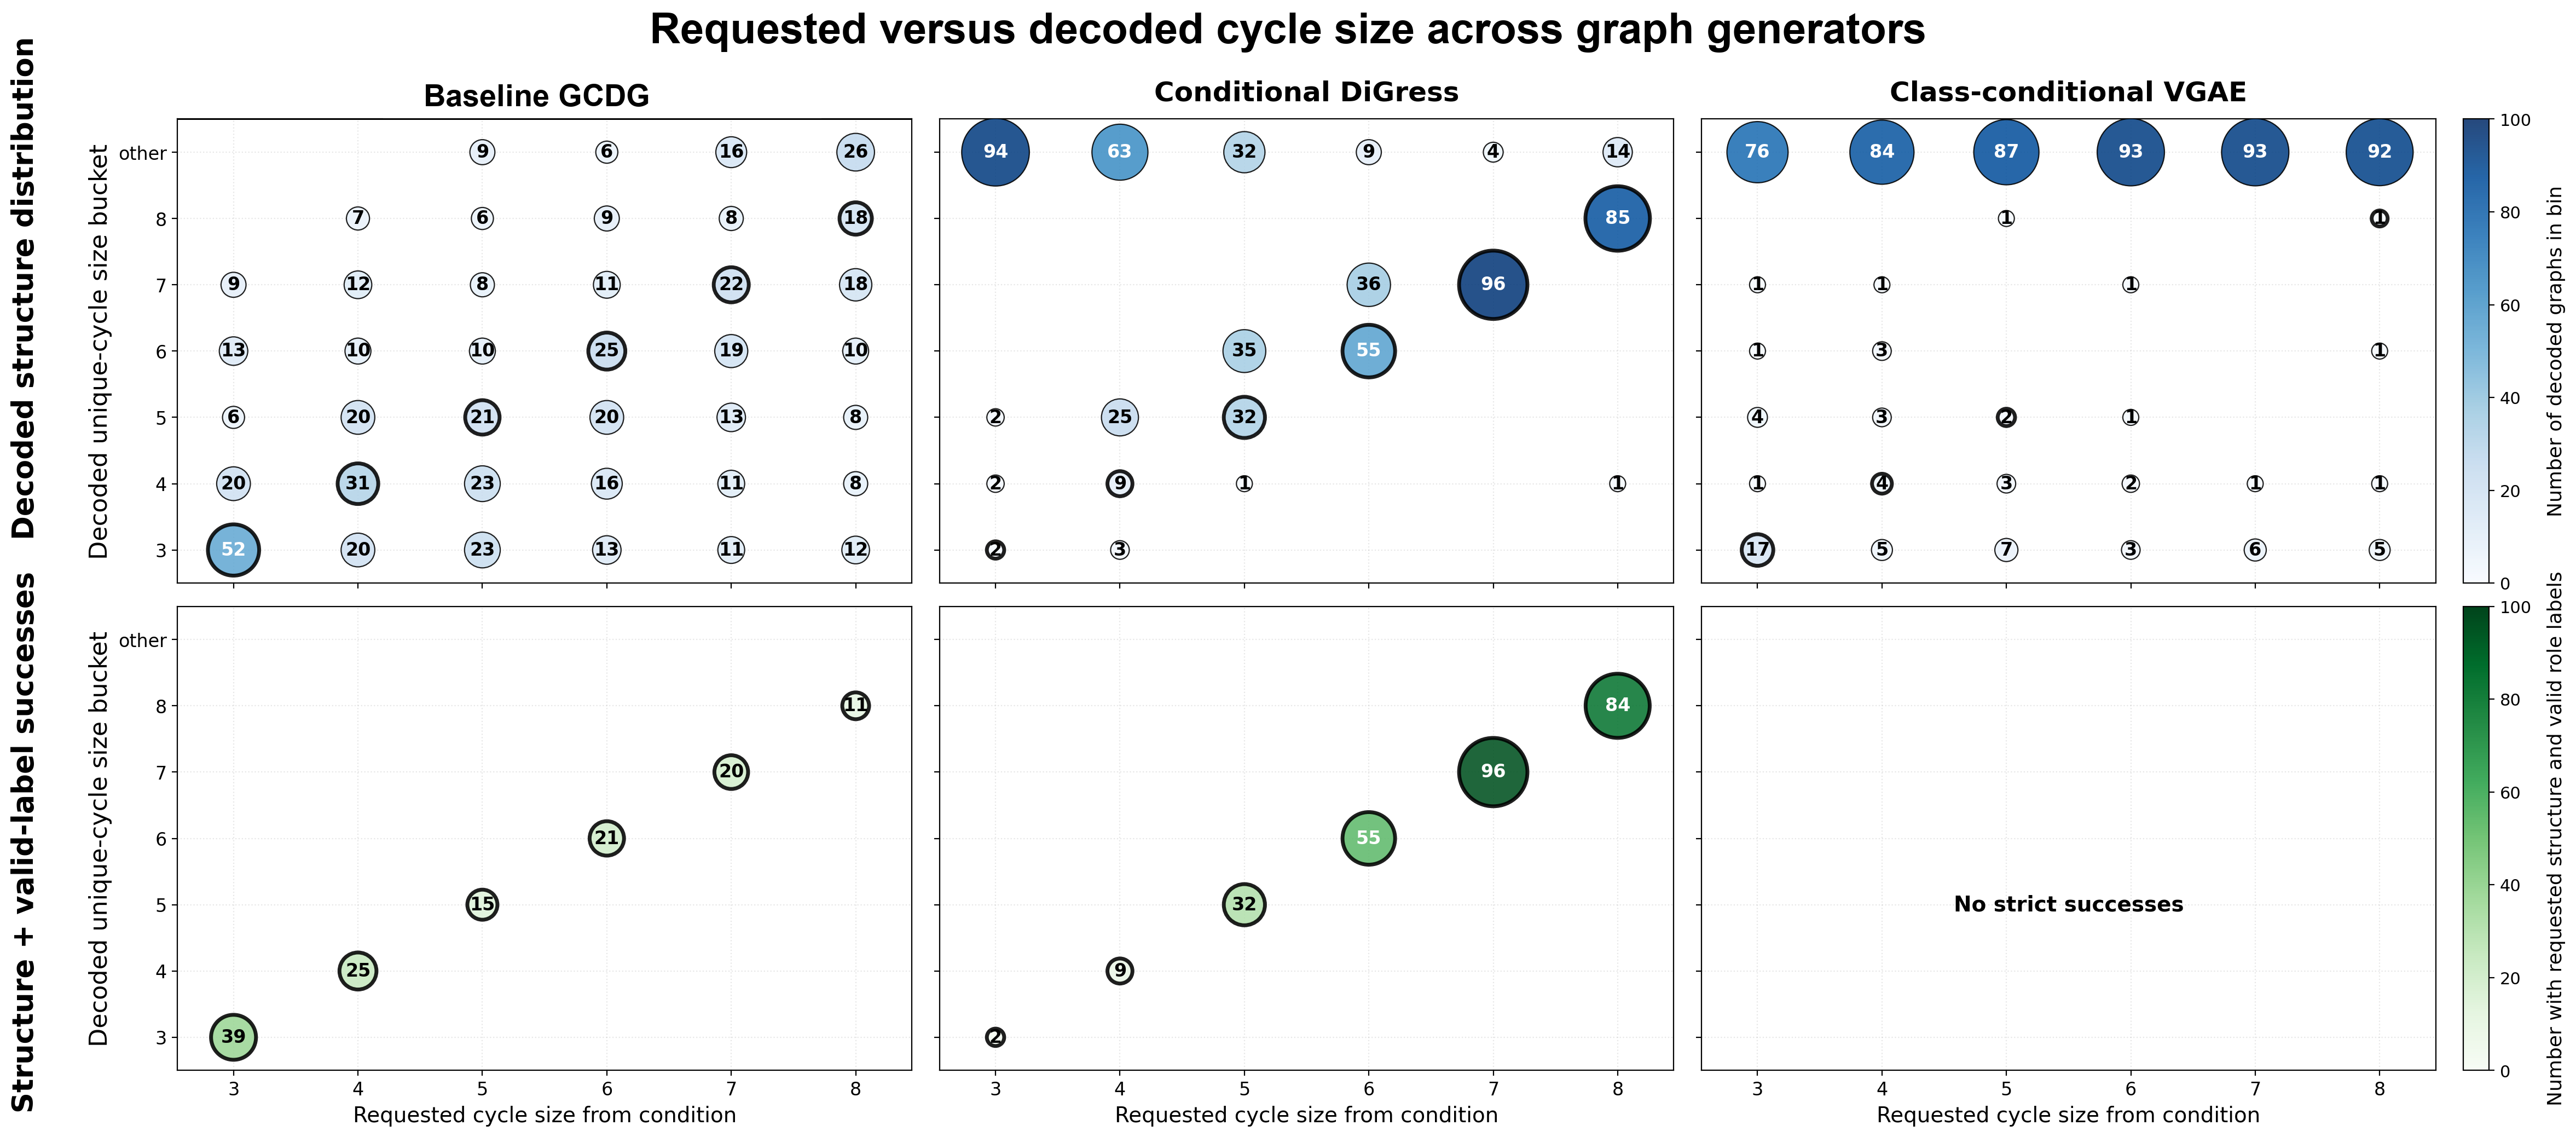
\includegraphics[
        width=1.2\textwidth,
        height=0.70\textheight,
        keepaspectratio
    ]{images/diffusion/req_vs_decoded_cycle.png}
    }
    \caption{
    Qualitative and aggregate results for the synthetic cycle--leg experiment.
    Top: examples of held-out condition graphs and generated outputs. These
    examples are illustrative; only nine generated graphs are shown for each
    displayed setting. Bottom: aggregate requested-versus-decoded cycle-size
    counts over all \(100\) generated samples per requested cycle size. In the
    bottom panel, the top row shows the decoded structure distribution and the
    bottom row counts strict successes where both the requested cycle size and
    role labels are correct. The \emph{other} bucket denotes outputs that do
    not have the required cycle--leg form, for example graphs with incoherent
    structure rather than a single cycle with one path attachment.
    }
    \label{fig:generator:req-vs-cycle-combined}
    \label{fig:generator:req-vs-gen-examples}
    \label{fig:generator:req-vs-decoded-cycle}
\end{figure}

Figure~\ref{fig:generator:req-vs-cycle-combined} first gives a qualitative view
of the experiment, showing examples of condition graphs and generated outputs.
The examples make the failure modes visually apparent, but they should not be
read as frequencies. The lower panel therefore reports the corresponding
aggregate counts out of \(100\) generated graphs per requested cycle size.

The aggregate counts show that the three models fail in different ways. The
GCDG has the broadest coverage of the cycle--leg family and
produces relatively few samples in the \emph{other} bucket. Its advantage is
clearest for the smallest requested cycles. For requested cycle sizes \(3\) and
\(4\), GCDG produces \(52\) and \(31\) exact structural matches, respectively,
compared with \(2\) and \(9\) for conditional DiGress. The same pattern appears
in the strict structure-plus-label counts: GCDG produces \(39\) and \(25\)
strict successes for cycle sizes \(3\) and \(4\), whereas conditional DiGress
produces \(2\) and \(9\).

Conditional DiGress shows the opposite behaviour. It places most cycle-three
and cycle-four requests in the \emph{other} bucket, but becomes very accurate
for larger requested cycles. For cycle sizes \(6\), \(7\), and \(8\), it
produces \(55\), \(96\), and \(84\) strict successes, respectively. GCDG still
often generates cycle--leg-like graphs for these larger conditions, but its
mass is spread across neighbouring cycle-size buckets rather than concentrated
on the requested size. The class-conditional \gls{vgae} baseline mostly
produces outputs in the \emph{other} bucket and has no strict successes,
indicating that class-level conditioning alone is not enough for this
graph-level conditional task.

This experiment isolates the role of the conditioning mechanism. A model can
generate plausible-looking graphs while still failing the conditional task. The
strict metric is therefore the rate of graphs that match both the requested
structure and the required label pattern, while the structure-distribution
panel is important for identifying whether failures remain within the intended
cycle--leg family or leave that family altogether.

\subsection{Molecular Conditional Generation}

The second set of experiments evaluates the same generator on molecular graphs.
Here the graph-level condition is computed from molecular graphs, and generation
is tested on held-out conditions not used for training. This setting asks
whether the generator can map a graph-level molecular description to a new
decoded molecular graph while maintaining chemical validity and distributional
similarity.

Generated molecules are compared with the held-out conditioning molecules that
produced them and with a reference sample from the training set. The molecular
analysis reported here focuses on two views. First, RDKit drawings provide a
qualitative inspection of generated molecular structure. Second,
distributional agreement is measured using scalar-property \gls{mmd} for
molecular weight, logP, QED, TPSA, density, atom count, bond count, and mean
bond degree. Additional validity, copying, novelty, and uniqueness diagnostics
were computed during the experimental workflow, but the main chapter reports
the RDKit visualisations and the distributional \gls{mmd} comparison.

The same held-out molecular condition set is used for the conditional
DiGress-style comparison. In both models, the condition is constructed in the
same way: a high-dimensional \gls{nsppk} graph feature vector is computed, a
truncated \gls{svd} projection fitted on the training graphs maps it to a
128-dimensional vector, and this fitted projection is then frozen and reused for
all held-out and generated graphs. Each held-out condition produces one
generated molecule. This makes the comparison a test of the generator rather
than a test of different condition vectors. The exact molecular dataset,
conditioning, training, and sampling settings are listed in
Appendix~\ref{app:qm9-molecular-settings}.

Because this is conditional generation, the evaluation also compares each
generated graph with the particular condition that produced it. For scalar graph
and molecular properties, condition-versus-generated scatter plots show whether
the generator preserves the requested property at the level of individual
conditions. For graph-level vector preservation, the generated graph is
re-encoded as \(\hat{C}\) and compared with the original condition \(C\) using
same-dimension correlations, pairwise cosine similarities, and pooled
condition-versus-re-encoding scatter plots.

\begin{figure}[t]
    \centering
    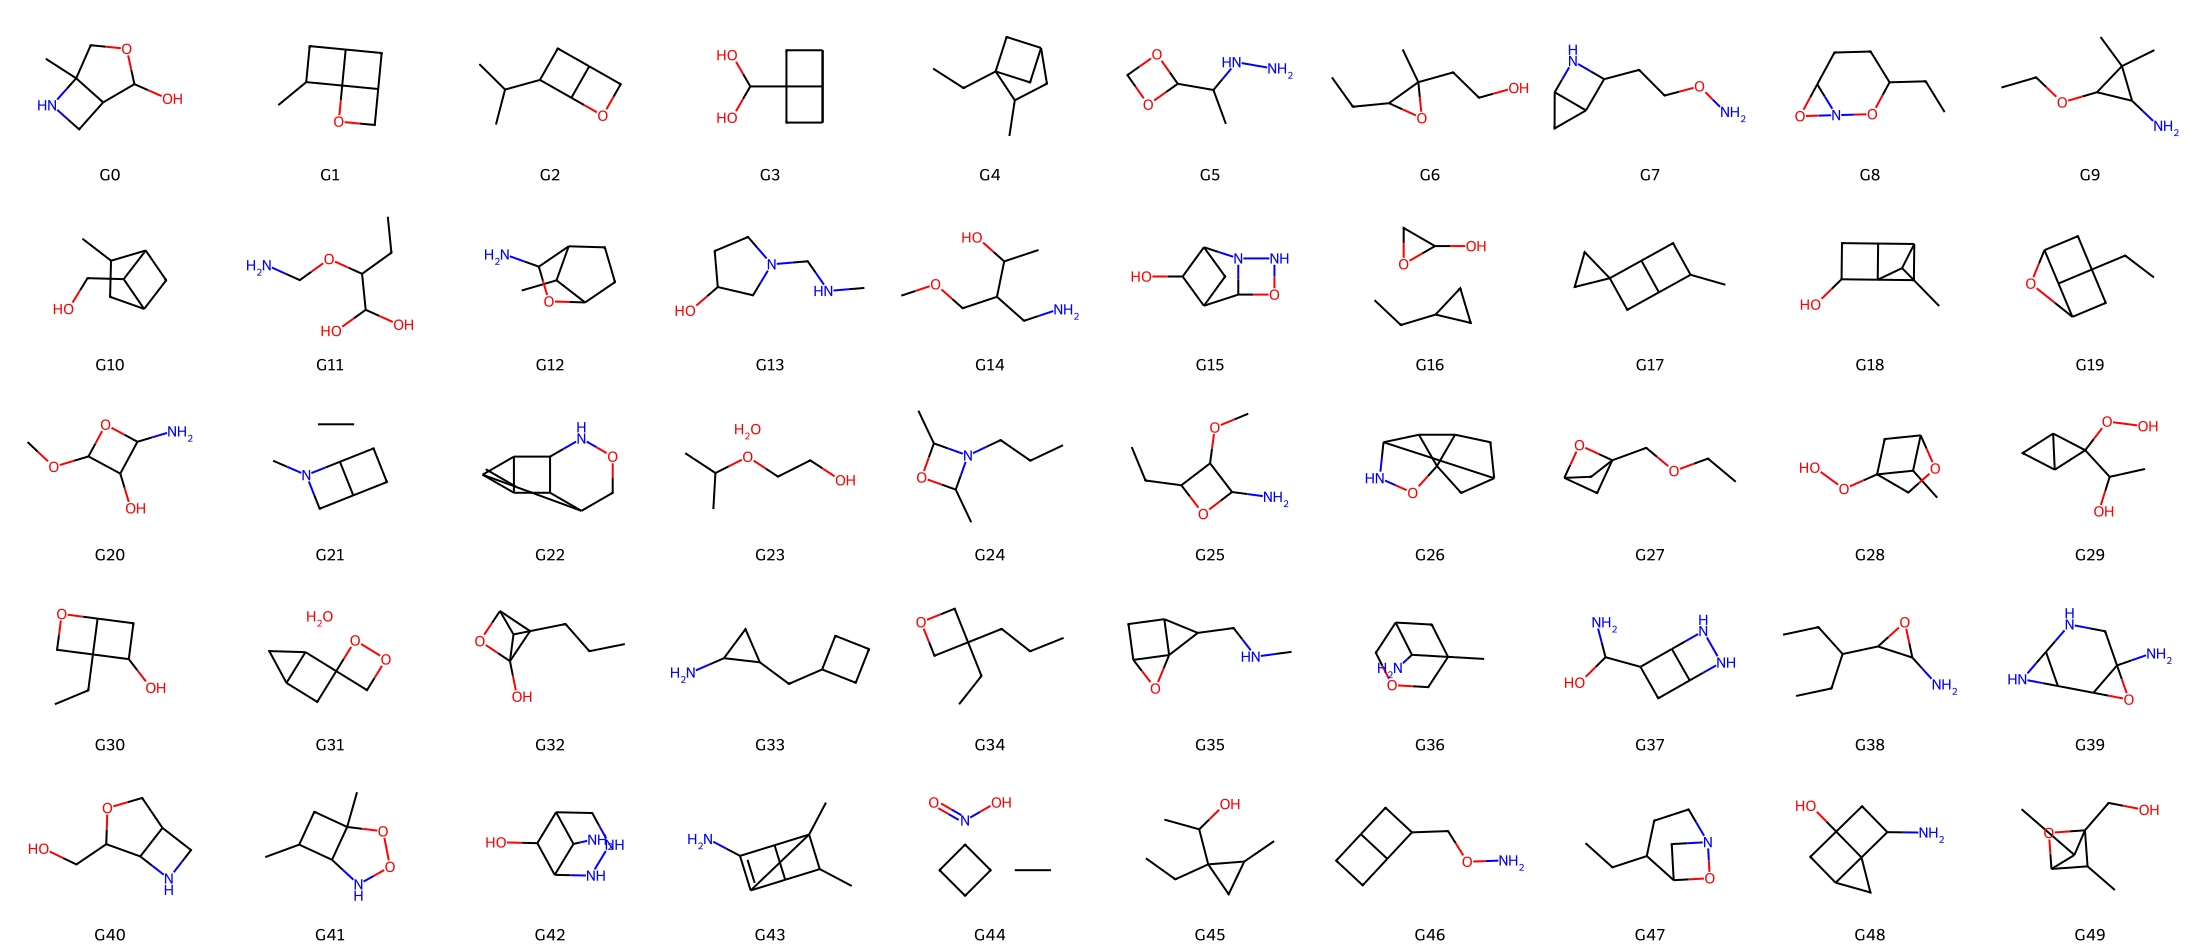
\includegraphics[
        width=\textwidth,
        keepaspectratio
    ]{images/diffusion/example_generated_my_generator.png}
    \caption{
    RDKit visualisations of QM9-like molecules generated by GCDG from held-out
    graph-level molecular conditions. These examples are qualitative samples;
    aggregate distributional comparisons are reported separately.
    }
    \label{fig:generator:qm9-gcddg-rdkit-examples}
\end{figure}



\begin{table}[t]
\centering
\footnotesize
\resizebox{\textwidth}{!}{%
\begin{tabular}{@{}lrrrrrrrr@{}}
\toprule
Model & Density & logP & Mean bond degree & Mol. weight & Bond count & Atom count & QED & TPSA \\
\midrule
GCDG & 0.006580 & 0.001988 & 0.000733 & 0.123563 & 0.008957 & 0.022764 & 0.075740 & 0.000935 \\
Conditional DiGress & 0.018580 & 0.001884 & 0.021891 & 0.010599 & 0.020499 & \(5.60\times10^{-7}\) & 0.000709 & 0.001297 \\
\bottomrule
\end{tabular}%
}
\caption{
Scalar-property \(\mathrm{MMD}^2\) between molecules generated from held-out
conditions and the held-out molecules that supplied those conditions. Smaller
values indicate closer agreement with the conditioning-molecule distribution.
Only the generated-versus-held-out-condition comparison is shown.
}
\label{tab:qm9-generated-vs-heldout-mmd}
\end{table}

Table~\ref{tab:qm9-generated-vs-heldout-mmd} shows complementary behaviour.
GCDG more closely matches structural graph statistics such as
density, mean bond degree, and bond count. Conditional DiGress more closely matches
molecular-size and chemistry-related descriptors such as atom count, molecular
weight, and QED.

\subsection{Synthetic Ablations}
\label{sec:generator:synthetic-ablations}

The synthetic cycle--leg task also provides a controlled setting for testing
which parts of the generator are needed for conditional graph construction. The
baseline setting is the Baseline GCDG configuration shown in the left column of
Figure~\ref{fig:generator:req-vs-cycle-combined} and specified in
Appendix Table~\ref{tab:synthetic-cycle-leg-proposed-hyperparameters}. Each
non-baseline ablation changes the named component and is evaluated using the
same \(100\) decoded graphs per requested cycle size. The exact cycle rate
counts graphs with the requested cycle size, while the stricter metric
additionally requires the node labels to match the required structural roles.
The Baseline GCDG row therefore corresponds to
the diagonal counts in the GCDG panels of
Figure~\ref{fig:generator:req-vs-cycle-combined}: \(169\) exact structural
matches and \(131\) strict structure-and-label matches out of \(600\) decoded
graphs.

\begin{table}[p]
\centering
\footnotesize
\begin{tabularx}{\textwidth}{@{}Xrr@{}}
\toprule
Configuration & Exact cycle rate & Strict rate \\
\midrule
Baseline GCDG & 0.282 & 0.218 \\
No degree-histogram control & 0.058 & 0.038 \\
No node-count control & 0.170 & 0.028 \\
No node-label histogram control & 0.242 & 0.110 \\
Matched-row loss enabled & 0.225 & 0.120 \\
Joint edge-state variant enabled & 0.155 & 0.017 \\
Random row permutation enabled & 0.248 & 0.168 \\
No distance supervision & 0.233 & 0.128 \\
Balanced degree loss enabled & 0.275 & 0.217 \\
No balanced edge loss & 0.280 & 0.197 \\
No node-feature dimensionality reduction & 0.175 & 0.005 \\
No clean-\(X_0\) reconstruction loss & 0.143 & 0.032 \\
No denoising-consistency loss & 0.297 & 0.235 \\
No balanced node-label loss & 0.250 & 0.162 \\
No node-label loss & 0.172 & 0.022 \\
No edge-existence loss & 0.125 & 0.008 \\
No node-existence loss & 0.217 & 0.120 \\
No degree loss & 0.163 & 0.007 \\
No edge supervision & 0.197 & 0.005 \\
No MST warm start & 0.203 & 0.095 \\
No connectivity constraint & 0.223 & 0.172 \\
No existence projection during sampling & 0.188 & 0.082 \\
No degree projection during sampling & 0.228 & 0.175 \\
No node-label projection during sampling & 0.193 & 0.050 \\
Degree and node-label channels denoised continuously & 0.243 & 0.155 \\
\bottomrule
\end{tabularx}
\caption{
Ablation results on the synthetic cycle--leg task. The Baseline GCDG row uses
the configuration specified in
Appendix Table~\ref{tab:synthetic-cycle-leg-proposed-hyperparameters}. Each
rate is computed over \(600\) decoded graphs:
\(100\) samples for each of the six requested cycle sizes. Exact cycle rate is
the fraction of decoded graphs that recover the requested cycle size, while
strict rate is the fraction that also recover the correct cycle and leg role
labels. Each non-baseline row changes the named component relative to the
Baseline GCDG configuration.
}
\label{tab:generator:synthetic-ablation-results}
\end{table}

Table~\ref{tab:generator:synthetic-ablation-results} shows that conditioning
controls and supervised structural heads have different effects. Removing the
degree-histogram control causes the largest drop in exact cycle recovery,
showing that the graph-level condition alone is not sufficient unless the
decoder is also supplied with a stable degree-composition target. Removing
node-count control, node-label histogram control, node-label supervision,
degree supervision, or the clean-\(X_0\) reconstruction loss mainly damages the
strict score, which means that the generator can still produce cycle-like
graphs but loses the alignment between structure and labels.
Removing distance supervision gives a smaller but still visible drop in both
rates, indicating that binned pairwise-distance targets help the model place
the requested cycle but are not the only structural signal used by the decoder.

The edge-supervision ablation is particularly informative. When edge
supervision is disabled, the learned pairwise edge-probability head is no
longer available and decoding falls back to degree-based edge scores. The
resulting graphs remain structurally feasible in a coarse sense: in the
recorded run all decoded graphs were connected, and the mean number of edges
matched the mean number of nodes in each requested category. However, the strict
rate falls from \(0.218\) to \(0.005\). This indicates that degree and
connectivity constraints can still force the decoder towards unicyclic graphs,
but they do not replace learned pairwise information about where the cycle and
leg edges should be placed or how labels should align with that structure.

Some components are less critical in this synthetic setting. Removing the
denoising-consistency loss slightly improves both reported rates, suggesting
that this auxiliary term is not necessary for the cycle--leg benchmark. Balanced
degree and edge losses also have small effects relative to the main structural
supervision terms. These ablations support the design used in the main
experiment: GCDG works best when the graph-level condition is coupled to
explicit node-count, degree, label, and pairwise-edge predictions before the
constraint-aware decoder constructs the final discrete graph.

\section{Limitations}
\label{sec:generator:limitations}

The staged design also introduces limitations. First, the quality of generation
depends on the node representation. If the node feature matrix does not contain enough
information to distinguish structurally important roles, the denoiser may match
global statistics while placing labels incorrectly. Second, the constrained
decoder can correct some structural inconsistencies, but it cannot recover
information that the denoiser failed to represent. Third, the integer
optimisation step improves feasibility but may become expensive for larger
graphs or dense candidate edge sets.

A further limitation is that chemistry-aware rules, when enabled, are not the
same as learning chemistry from data alone. Valency projection can improve
RDKit validity by removing or downgrading invalid bonds, but this should be
reported as a post-processing constraint rather than as unconstrained neural
generation. Similarly, dynamic molecular features provide the denoiser with
state-dependent chemical summaries; they are appropriate for molecular
ablations but are not part of the generic graph generator.

Finally, the model is conditional on a graph-level vector \(C\). Strong
conditioning performance therefore depends on the informativeness and stability
of this vector. In the experiments, condition consistency is assessed through
proxy comparisons with the held-out graphs that supplied the condition:
structural statistics, molecular properties, and correlations between the
condition vector \(C\) and the re-encoded generated graph \(\hat{C}\). These
comparisons test whether the generated graph preserves information encoded in
the condition, rather than whether it reconstructs the conditioning graph
exactly.

\section{Summary}
\label{sec:generator:summary}

This chapter introduced the Graph-Conditioned Diffusion Generator, a
conditional graph generator that maps a fixed graph-level descriptor to a
discrete labelled graph. The method separates the continuous reverse diffusion
process over padded node features from the later decisions that determine node
existence, node labels, degree classes, edge probabilities, and edge labels.
The final graph is obtained by a constraint-aware decoder, so graph feasibility
is handled explicitly rather than being left entirely to the neural denoising
network.

The synthetic cycle--leg experiment shows why this staging is useful. The model
does not merely generate plausible graphs; it can be evaluated against explicit
conditional requirements such as requested cycle size and role-label placement.
The comparison with conditional DiGress and a class-conditional \gls{vgae}
baseline shows that different generators fail in different ways: GCDG performs
best on the smallest requested cycles and produces fewer samples outside the
intended cycle--leg family, whereas DiGress is much stronger on the larger
requested cycles.

The QM9 experiment extends the same conditioning mechanism to molecular graphs.
In this chapter, the molecular results are reported through RDKit
visualisations and scalar-property \gls{mmd} comparisons between generated
molecules and the held-out molecules that supplied their conditions. 
The results should be interpreted as a conditional distributional comparison
rather than as a complete molecular benchmark. They show that GCDG
matches some structural graph statistics closely, whereas the conditional
DiGress-style model better matches molecular-size and chemistry-related
descriptors such as atom count, molecular weight, and QED.

Overall, the chapter establishes GCDG as a graph-conditioned diffusion
generator in which continuous node-feature generation and discrete graph
construction are deliberately separated. The experiments show that this design
can preserve explicit conditional structure in the synthetic setting, while the
molecular setting exposes the additional difficulty of matching chemical and
property-level constraints. These results motivate the next chapter, which
turns from generator design to the broader problem of evaluating generated data
with diagnostic, statistically grounded probes.
